\documentclass[11pt, oneside]{article}   	% use "amsart" instead of "article" for AMSLaTeX format
\usepackage{geometry}                		% See geometry.pdf to learn the layout options. There are lots.
\geometry{letterpaper}                   		% ... or a4paper or a5paper or ... 

\usepackage[english]{babel}
\usepackage{url, verse}
\usepackage{pstricks, tikz}
\usepackage[T1]{fontenc}
\usepackage{setspace}
\usepackage{graphicx, wrapfig, capt-of}
\usepackage[normalem]{ulem} %for \sout
\usepackage{amssymb}
\usepackage{color}
\usepackage{tipa}
\usepackage{multicol}
\raggedcolumns

\usepackage{stackengine}
\usepackage{array}
\newcolumntype{P}[1]{>{\centering\arraybackslash}p{#1}}
\newcolumntype{M}[1]{>{\centering\arraybackslash}m{#1}}
\usepackage{hhline,multirow, chngpage}
\newcommand*\rot{\rotatebox{90}}

\usepackage{linguex} %declare this package after tipa and graphicx
\renewcommand{\firstrefdash}{}
\usepackage{qtree}
%\usepackage{tree-dvips} %copy tree-dvips folder to make this work
\qtreecenterfalse

\usepackage{float}
\usepackage{tcolorbox, enumitem}
\usepackage{phonrule}

\usepackage{fancyhdr}
\pagestyle{fancy}{
\fancyhead[L]{Roberto Petrosino}
\fancyhead[C]{LING2010Q}
\fancyhead[R]{4: Morphology}
\renewcommand{\footrulewidth}{0pt}
\renewcommand{\headrulewidth}{0pt}}

\newenvironment{packed_enum}{
\begin{enumerate}
  \setlength{\itemsep}{1pt}
  \setlength{\parskip}{0pt}
  \setlength{\parsep}{0pt}
}{\end{enumerate}}

\newenvironment{packed_item}{
\begin{itemize}
  \setlength{\itemsep}{1pt}
  \setlength{\parskip}{0pt}
  \setlength{\parsep}{0pt}
}{\end{itemize}}

\renewcommand{\labelitemiii}{$\diamond$}


\title{{\normalsize LING 2010Q -- {\scshape Fall 2017}} \\ {\bfseries 4 - Morphology}, or: \\ {\itshape what words are made of}}
\author{Roberto Petrosino \hspace{0.2cm} \url{roberto.petrosino@uconn.edu}}
\date{Oct 5-Oct 17, 2017}

\begin{document}

\maketitle
\vspace{-1cm}
{\small \tableofcontents}

\newpage

\section{(Falling into) Pieces}

\subsection{Activity 1a: What are words made of?}\label{act:words}

{\itshape Consider the following words and identify how many pieces of information they are made of. Can you detect them all? :)}

\setlength\columnsep{0.5pt}
\begin{multicols}{5}
\centering
\scriptsize
\begin{itemize}
\item Massachussetts
\item dog
\item government

\columnbreak

\item thinks
\item electricity
\item erasure

\columnbreak

\item bookshelf
\item tremendous
\item assumption

\columnbreak

\item carefully
\item astonish
\item computer

\columnbreak

\item unidirectional
\item department
\item under

\end{itemize}
\end{multicols}

\ex. A {\bfseries morpheme} is the {\itshape minimal meaningful unit} in a language. Words are made of at least one morpheme. 
	\a. Mono-morphemic words are called {\bfseries free morphemes}, because they can stand on their own, and cannot be further broken down.
	\b. Pluri-morphemic words are made of more than one morpheme; each of them are therefore {\bfseries bound}.

\subsection{Activity 1b: Morphemes}

{\itshape List the morphemes detected in Activity \ref{act:words} in the gaps. Are they free or bound? Check the appropriate box.}

%%%%%%%%%

\ex. {\bfseries Affixes} are morphemes that are always ``bound'' (i.e., attached) to the root, which is the morpheme carrying the core meaning. Depending where they attach to the root, they may be called:
	\a. {\itshape prefixes}
	\b. {\itshape suffixes}
	\c. {\itshape infixes}

\ex. There are also {\itshape bound roots}, though rare in English: e.g., \underline{cran}-berry, \underline{scissor}-s.

\subsection{Activity 2: Spanish}

{\itshape The following data are from Spanish. Identify all the morphemes present, and state the meaning and/or function of each morpheme.}

\begin{center}
\begin{tabular}{l l | l l}
amigo & `male friend'	&	muchachas	& `children (girls)' \\
amigos & `male friends'	&	muchacha	&	`child (girl)'	\\
amigas & `female friends' & muchachos	& `children (boys)' \\
muchacho & `child (boy)' & amiga	&	`female friend' \\
\end{tabular}
\end{center}

\subsection{Activity 3: Persian}

{\itshape The following examples are from Persian. Try to match the meanings in a) through h> with a morpheme in the Persian data. Mark prefixes with a hyphen following the morpheme (X-), and suffixes with a hyphen preceding the morpheme (-X).}

\begin{center}
\begin{tabular}{l l}
{[}xarid]		&	`bought' \\
{[}mixarid]	& 	`was buying' \\	
{[}xaridam]	& 	`I bought' \\
{[}xaridi]	&	`You (sg) bought' \\
{[}mixaridid]	&	`You (pl) were buying' \\
{[}naxaridam]	&	`I did not buy' \\
{[}namixaridand] &	`They were not buying' \\
{[}naxaridim]		&	`We did not buy' \\
\end{tabular}
\end{center}

\begin{tabular}{l l l l}
I 			& 	\underline{\hspace{1cm}}	&      	they 		&	\underline{\hspace{1cm}} \\	
you(sg) 	& 	\underline{\hspace{1cm}}				&		not  		&	\underline{\hspace{1cm}} \\
we			& 	\underline{\hspace{1cm}} 			&		Progressive &	\underline{\hspace{1cm}} \\
you (pl) 	&	\underline{\hspace{1cm}}				&		buy + PAST 	&	\underline{\hspace{1cm}} \\
\end{tabular}

\vspace{0.5cm}

\noindent {\itshape How would you say the following sentences in Persian?}

\vspace{0.2cm}

\begin{tabular}{l l}
They were buying 	& 	\underline{\hspace{1cm}} \\
You(sg) did not buy &	\underline{\hspace{1cm}} \\
You(pl) were buying &	\underline{\hspace{1cm}} \\
\end{tabular}

\ex. {\itshape Morphemes} and {\itshape syllables} are {\itshape \bfseries NOT} the same thing! See slides for more info.

\subsection{Categories}

\ex. Affix may be grouped into {\scshape classes} when they share:
\a. the syntactic category of the root that they attach to
\b. the category of the whole word created
\c. the meaning/information carried by the morpheme. For example:

\begin{center}
\begin{tabular}{l l l l l} \hline
The affix & attaches to & forms & means & example \\ \hline
un- &	Adjective	&	Adjective	& `not' &	un-friendly \\ 
	&	Verb		&	Verb		& `reverse'	& un-button \\
-ize &	Adjective	&	Verb		& `to make Adj' & stabil-ize \\
-er	&	Adjective	&	Adjective	& `more'	&	tall-er \\
\end{tabular}
\end{center}

\newpage

\ex. {\scshape Syntactic categories} express the role of words in a sentence. The main syntactic categories we will be looking at are:
\a. {\scshape noun}
\b. {\scshape verb}
\c. {\scshape adjective}
\d. {\scshape adverb}
\e. {\scshape preposition}

\subsubsection{Activity 4: Categories (I)}

{\itshape Consider the following lists of words:}

\begin{enumerate}
\item incorrigible, incongruous, indefinite, inflexible, insurmountable
\item cowardly, daily, fatherly, friendly, lonely, lovely, womanly
\item dependent, descendant, defiant, prudent, reverent, servant
\end{enumerate}

\noindent {\itshape In each list, is there a morpheme all the words have in common?  If so, give three more words that contain that morpheme and give the meaning of the morpheme.  What syntactic category does the morpheme attach to?  What syntactic category does the resulting word belong to:?}

\ex. The class of words can also be defined in terms of the affixes they can combine with. For example, the following generalizations are true of English:
\a. Only {\scshape nouns} can take the plural marker {\itshape -s}: book-s, *tall-s
\b. Only {\scshape adjectives} have comparative forms, {\itshape -er}: tall-er, *book-er
\c. Only {\scshape verbs} have past forms, {\itshape -ed}: talk-ed, *tall-ed

\ex. Note that not all nouns have a regular plural in {\itshape -s} (e.g., goose/geese), not all adjectives have a comparative in {\itshape -er} (e.g., bad/worse), not all verbs have an {\itshape -ed} for the past (e.g., speak/spoke).  These forms are irregular (see secc. \ref{allomorphy} and \ref{strategies} further below).

\ex. An {\bfseries open} morpheme class is one that freely takes new members, e.g., nouns, verbs, adjective.  A {\bfseries closed} morpheme class is one that does not allow new members; most affix classes are like this.

\newpage

\subsubsection{Activity 5: Categories (II)}

{\itshape Fill in the right syntactic category for each of the following words.} \\

\begin{tabular}{r l l}
act -- active: & \underline{\hspace{1cm}} + -ive & becomes \underline{\hspace{1cm}} \\
active -- activate:	& \underline{\hspace{1cm}} + -ate & becomes \underline{\hspace{1cm}} \\	                    
activate - deactivate: & de- + \underline{\hspace{1cm}} & remains \underline{\hspace{1cm}} \\         
deactivate - deactivation:	& \underline{\hspace{1cm}} + -ion & becomes \underline{\hspace{1cm}} \\
\end{tabular}

\ex. A {\scshape paradigm} is a set of all forms which contain a common element, especially the set of all inflectional forms of a word or a particular grammatical category ({\em simplified}).
	\a.[] e.g.: {\em go $\sim$ went $\sim$ gone} is the paradigm of the verb `to go'.

\ex. {\scshape Inflectional} categories in languages:
\a. {\bf Number}: attaches to nouns, indicates quantity
	\a.[] Samoan: {\it \textipa{P}oe} `you (singular)',  {\it \textipa{P}oulua} `you (dual)', {\it \textipa{P}outou} `you (plural)'
	\z.  
\b. {\bf Gender}: attaches to nouns (adjective)
	\a.[] Spanish: {\it l-o-s muchach-o-s mexican-o-s} $\sim$ {\it l-a-s muchach-a-s mexican-a-s}
	\z.
\c. {\bf Case}: attaches to nouns (adjective), marks grammatical function
	\a.[] English: {\it we} (nominative), {\it us} (accusative), {\it our} (possessive)
	\b.[] Finnish: {\it talo-} `house'
	
\begin{center}	
\begin{tabular}{l l | l l}
{\itshape nominative}	&	talo &	{\itshape allative} (`to') & talo-lle\\
{\itshape accusative}	&	talo-n & {\itshape essive} (`at') & talo-na \\
{\itshape genitive (`of')}	&	talo-n & {\itshape partitive} (`part of')	& talo-a \\
{\itshape inessive} (`in')	& talo-ssa & {\itshape translative} (`change to') & talo-ksi \\
{\itshape elative} (`out of')	&	talo-sta & {\itshape abessive} (`w/o')	& talo-tta \\
{\itshape illative} (`in')	& talo-on & {\itshape instructive} (`by') & talo-in \\
{\itshape adessive} (`on')	& talo-lla & {\itshape comitative} (`w/') & talo-ine \\
\end{tabular}
\end{center}
	
\ex.[] 
\a.[d.] {\bf Person}: attaches to nouns/verbs, marks role of referent in conversation
	\a.[] Old English: {\it folgie} (1st), {\it folgast} (2nd), {\it folgaþ} (3rd) `follow'
	\z.
\b.[e] {\bf Tense}: attaches to verbs, indicates time of event
	\a.[] French: {\it il parle} `he speaks', {\it il parlera} `he will speak'
	\z.
\c.[f] {\bf Aspect}: attaches to verbs, marks point of view of event
	\a.[] Russian:
		\a.[] {\it ja pro{\v c}ital roman} `I finished reading the book'
		\b.[] {\it ja {\v c}ital roman} `I read from the book'
		\z.
	\z.
\d.[g.] {\bf Mood}: attaches to verbs, marks actuality/possibility
	\a.[] Luise{\~ n}o: 
		\a.[] {\it n{\' o}o \textipa{N}aaq} `I am leaving'
		\b.[] {\it noo n{\' e}evi{\v c}uq} `I want to leave'
		\z.
	\z.
\e.[h.] {\bf Voice}: attaches to verbs, marks who performs an action
	\a.[] Latin: 	
		\a.[] {\it puella amat} `the girl loves'
		\b.[] {\it puella amatur} `the girl is loved'
		\z.
	\z.
 
\subsubsection{Activity 6: Morpho-drills}

{\itshape Answer the following questions.}

\begin{enumerate}
\item How many morphemes are there in each of the following words?
	\begin{enumerate}
	\item {\it sweeter}: 
	\item {\it eaten}:
	\item {\it sweetener}:
	\end{enumerate}
\item Determine the syntactic category of the roots and complex words in these examples.
	\begin{enumerate}
	\item {\it sweeter}: 
		\begin{itemize}
		\item {\em root:} \underline{\hspace{1cm}}; {\em category:} \underline{\hspace{1cm}}
		\item {\em word:} \underline{\hspace{1cm}}; {\em category:} \underline{\hspace{1cm}}
		\end{itemize}
	\item {\it eaten}:
		\begin{itemize}
		\item {\em root:} \underline{\hspace{1cm}}; {\em category:} \underline{\hspace{1cm}}
		\item {\em word:} \underline{\hspace{1cm}}; {\em category:} \underline{\hspace{1cm}}
		\end{itemize}
	\item {\it sweetener}:
		\begin{itemize}
		\item {\em root:} \underline{\hspace{1cm}}; {\em category:} \underline{\hspace{1cm}}
		\item {\em word:} \underline{\hspace{1cm}}; {\em category:} \underline{\hspace{1cm}}
		\end{itemize}
	\end{enumerate}
\item Give the meaning of each affix and state whether it refers to an inflectional category or not.
	\begin{multicols}{3}
	\begin{enumerate}
	\item \underline{\hspace{1cm}}: 
		\begin{itemize}
		\item {\em meaning:} \underline{\hspace{1cm}}
		\item Inflectional? Y \hspace{0.5cm} N
		\end{itemize}
	\columnbreak
	\item \underline{\hspace{1cm}}:
		\begin{itemize}
		\item {\em meaning:} \underline{\hspace{1cm}}
		\item Inflectional? Y \hspace{0.5cm} N
		\end{itemize}
	\columnbreak
	\item \underline{\hspace{1cm}}:
		\begin{itemize}
		\item {\em meaning:} \underline{\hspace{1cm}}
		\item Inflectional? Y \hspace{0.5cm} N
		\end{itemize}
	\end{enumerate}
	\end{multicols}
\end{enumerate}

\newpage

\subsubsection{Activity 7: English affixes}

{\itshape From the examples given for each of the following suffixes, determine: i) the syntactic category of the root, and ii) the syntactic category of the word resulting from the addition of the suffix.} \\

\medskip %add some space
\begin{adjustwidth}{-0.4in}{-0.4in}% adjust the L and R margins by 1 inch
\begin{tabular}{l l l l l}
a. & -ify	&	solidify, intensify, purify, clarify, rarefy	&	-ify takes \underline{\hspace{1cm}} & and yields \underline{\hspace{1cm}} \\
b. & -ity	&	rigidity, stupidity, hostility, intensity, responsibility	& -ity takes \underline{\hspace{1cm}} & and yields \underline{\hspace{1cm}} \\
c. & -ize:	& unionize, terrorize, hospitalize, crystallize, magnetize	& -ize takes \underline{\hspace{1cm}} & and yields \underline{\hspace{1cm}} \\
d.	& -ive & repressive, active, disruptive, abusive, explosive & -ive takes \underline{\hspace{1cm}} & and yields \underline{\hspace{1cm}} \\
e. &-ion &invention, injection, narration, expression, pollution & -ion takes \underline{\hspace{1cm}} & and yields \underline{\hspace{1cm}} \\
f. & -less & nameless, penniless, useless, heartless, mindless & -less takes \underline{\hspace{1cm}} & and yields \underline{\hspace{1cm}} \\
\end{tabular}
\end{adjustwidth}
\medskip %add some space

\subsection{Typology}

\ex. {\bfseries Analytic languages} have little morphology. For example, in Vietnamese:
\ag. Hai \textcrd ú.a bo\textsuperscript{\textipa{P}} nhau la tai gia-\textcrd inh thàng chông. \\
two people leave reciprocal be because family guy husband \\
`They divorced because of his family.'	

\ex. {\bfseries Synthetic languages} make extensive use of morphology. 
\a. In agglutinative languages the ratio `no. of morpheme: no. of morphological information' is always (1:1). For example:
	\ag.[] Marf-adi wi{\v c}i qalin st'al-ra-ldi qaw gata-zwa-j \\
	rain-{\scshape subj} self-of dense drop-s-with roof hit-ing-was \\
	`The rain is hitting the roof with its dense drops.' \hfill (Lezgian)                        
	\z.
\b. {\itshape Fusional languages} are synthetic languages that have morphemes, each of which may carry more than one piece of morphological information; for example, in Italian:
	\ag.[] Il gatt-o cattur-ò il top-o. \\
	\small The cat-{\scshape masc.sg} catch-{\scshape past.3sg} the mouse-{\scshape masc.sg} \\
	`The cat caught the mouse.'

\ex. Polysyntethic languages are agglutinative languages with extraordinary amounts of morphology, such that they can merge a sentence in a single word. 
\ag.[] paasi-nngil-luinnar-para 	ilaa-juma-sutit \\
understand-not-complete-{\scshape I.subj.it.3sg.ind}   come-want-you.{\scshape part} \\
`I didn't understand at all that you wanted to come.' \hfill (Greenlandic Eskimo)

\section{Allomorphy}\label{allormophy}

\subsection{Free vs conditioned allomorphy}

\ex. When the same morphological information is conveyed by more than one form, we say that that morpheme shows {\bfseries allomorphy}. There may or may not be conditions on where each of the allomorph shows up.  If either allomorph may show up wherever the other does, then they display {\bfseries free variation}. For example, in Zapotec (spoken in Mexico):

\begin{figure}[H]
\centering
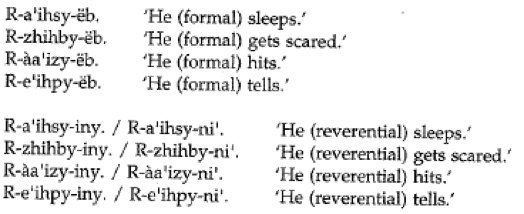
\includegraphics{zapotec.png}
\end{figure}%

%\newpage

\ex. If certain allomorphs only show up in certain restricted environments, then they display {\bfseries conditioned allomorphy}. For example, in English: 

\begin{multicols}{3}
\centering
\noindent impossible \\ 
immature \\
imbalanced \\
inactive \\
\columnbreak
indecent \\
intangible \\
illegal \\
illegible \\
\columnbreak
illogical \\
irreverent \\
irresponsible \\
irredeemable \\
\end{multicols}

\ex.[] In the cases above, what determines what allomorph to choose between {\itshape in-, im-, il- and ir-}? \\

{\it Your answer:} 
\vspace{1cm}


\subsection{Portmanteaux and suppletion}

\ex. Unfortunately, morphological analysis is not always that straightforward. On the one hand, languages may have some morpheme conveying more than one meaning; this phenomenon is called {\bfseries portmanteau} (or {\itshape suppletion}). %%%%

\subsubsection{Activity 8: Lakota.}

{\itshape Consider the following forms of Lakota, a Siouan language spoken in North and South Dakota. Identify all the morphemes contained, and ask the questions below.}

\vspace{0.2cm}

\begin{tabular}{l l}
pajája &	`he washed him' \\
wapájaja &	`I washed him' \\
yapájaja &	`you washed him' \\
mapájaja &	`he washed me' \\
nipájaja &	`he washed you' \\
\end{tabular}

\begin{enumerate}
{\itshape
\item Identify and gloss the lexical and grammatical morphemes above.
\item How are third person subjects and objects marked?
\item Consider the additional sentences below:}
		\begin{quote}
		\begin{tabular}{l l}
		mayápajaja & `you washed me' \\
		chipájaja & `I washed you' \\
		\end{tabular}
		\end{quote}
{\itshape Given the table above what you have expected the second sentence to be? \\
Your answer: 
\vspace{1cm}
\item What does {\normalfont chi-} mean? \\
Your answer:} \vspace{1cm}

\end{enumerate}

\ex. Sometimes different pieces of morphological information are conveyed by different forms unrelated to each other. This phenomenon is referred to as suppletion. For example, English:
	\a. go $\sim$ went, {\itshape but} love $\sim$ \underline{\hspace{1cm}}
	\b. I am $\sim$ you \underline{\hspace{1cm}} $\sim$ he/she/it \underline{\hspace{1cm}}, {\itshape but} I love $\sim$ he/she/it \underline{\hspace{1cm}}
	\c. I was $\sim$ you \underline{\hspace{1cm}}, {\itshape but} I type-d $\sim$ you \underline{\hspace{1cm}}
	\d. good $\sim$ better $\sim$ \underline{\hspace{1cm}}, {\itshape but} smart $\sim$ \underline{\hspace{1cm}} $\sim$ smart-est
	
\newpage
	
\section{Some (cool) morphological strategies}\label{strategies}

\subsection{Activity 8: Southern Paiute}

{\itshape Consider some data from Southern Paiute, spoken in Arizona, Nevada and Utah, and analyze it.}

\begin{center}
\begin{tabular}{l l l}
Noun	&	Verb	& 	Object incorporation \\
paa `water'	&	tu'uma `to take'	&	paaruiuma `to take water' \\
			&	pïni `to see'		&	paavïni `to see water' \\
qwo'a-ppi `tobacco'  &	tïqa `to eat'	&	qwo'attïqa `to smoke' \\
pagïu `fish'	&						&	pagïurïqa `to eat fish' \\
quqqwa-ppi `wood' &	pïga `to keep' 	&	quqqwappïqa `to gather wood' \\
\end{tabular}
\end{center}

\ex. Some language may {\bfseries incorporate} the object inside the verb, thus forming a single word.

\subsection{Activity 9: English (I)}

{\itshape Consider some data from English and analyze it with a colleague. Which syntactic category (i.e., Noun, Verb, Adjective, Adverb, Preposition) do each compound and and its parts belong to? }

\begin{enumerate}
\begin{multicols}{2}
\item lipstick (\underline{\hspace{0.5cm}} + \underline{\hspace{0.5cm}} = \underline{\hspace{0.5cm}})	
\item hardware (\underline{\hspace{0.5cm}} + \underline{\hspace{0.5cm}} = \underline{\hspace{0.5cm}})		
\item drawbridge (\underline{\hspace{0.5cm}} + \underline{\hspace{0.5cm}} = \underline{\hspace{0.5cm}})		

\columnbreak

\item babysit (\underline{\hspace{0.5cm}} + \underline{\hspace{0.5cm}} = \underline{\hspace{0.5cm}})
\item leadfree (\underline{\hspace{0.5cm}} + \underline{\hspace{0.5cm}} = \underline{\hspace{0.5cm}})
\item bittersweet (\underline{\hspace{0.5cm}} + \underline{\hspace{0.5cm}} = \underline{\hspace{0.5cm}})

\end{multicols}
\end{enumerate}

\noindent {\itshape Do you observe some consistency concerning the syntactic category of a compound and the syntactic categories of its components?\\
Your answer:} \vspace{1cm}

\newpage

\subsection{Activity 10: Ilocano}

{\itshape Consider some data from Ilocano. spoken in the Philippines, and analyze it.}\\

\begin{tabular}{l l | l l}
pí\textipa{N}gan &	`dish'		&	pi\textipa{N}pí\textipa{N}gan	&	`dishes' \\
tálon	& `field'		&	taltálon	&	`fields' \\
dálan	& `road'		&	daldálan	&	`roads' \\
bíag	& `life'		&	bibíag		&	`lives' \\
nuá	& `carabao'		&	nunuá		&	`carabaos' \\
úlo	& `head'		&	ulúlo		&	`heads' \\
\end{tabular}

\ex. {\bfseries Reduplication} is the process in which part or all of the root is copied. The reduplicated segment may occur as a {\itshape prefix, infix or suffix}.

\subsection{Activity 11: English (2)}

{\itshape Consider some data from English and analyze it. How is the relevant morphological information conveyed in these forms?}

\begin{center}
\begin{tabular}{l l || l l}
plural	&	cf.		& 	past	&	cf. \\ \hline
goose $\sim$ geese	&	dog $\sim$ dog-s	&	write $\sim$ wrote & type $\sim$ type-(e)d \\
mouse $\sim$ mice	&	cat $\sim$ cat-s	&	see $\sim$ saw 	&	look $\sim$ look-ed \\
man $\sim$ men 	&	kid $\sim$ kid-s	&	run $\sim$ ran	&	walk $\sim$ walk-ed \\
foot $\sim$ feet	&	shoe $\sim$ shoe-s	&	fall $\sim$ fell	&	drop $\sim$ drop(p)-ed \\
tooth $\sim$ teeth	&	lip $\sim$ lip-s	&	give $\sim$ gave	&	offer $\sim$ offer-ed \\
\end{tabular}
\end{center}

\ex. {\bfseries Ablaut} (also called apophony) is the morphological process involving change of the root vowel, rather than affixation, to convey certain morphological information.

\subsection{Activity 11: Chickasaw}

{\itshape Consider some data from Chickasaw, spoken in Oklahoma, and analyze it.}

\begin{center}
\begin{tabular}{l l l l}
sachaaha     &	`I am tall'	&	chichchokwa   &    `You are cold' \\
chaaha        & `He/she is tall'     &    	hopobatok         &      `He was hungry' \\
chichaaha     &       `You are tall'     &         	hoohopobatok  &   `They were hungry' \\
satikahbi      &        `I am tired'      &              sahopoba &         `I am hungry'\\
\end{tabular}
\end{center}

{\itshape What would you predict to be the form for `he was tired' and `he is hungry'?\\
Your answer:} \vspace{1cm}

{\itshape What would you suggest is the morpheme for `he'?\\
Your answer:} \vspace{1cm}

{\itshape Look at the following data, and use it to bear on your analysis.}

\begin{center}
\begin{tabular}{l l l l}
Chaaha sa-banna 	&	`I want to be tall' \\
Chaaha chi-banna	& 	`You want to be tall'\\
Chahha banna		&	`S/he wants to be tall'\\
\end{tabular}
\end{center}

\ex. Languages may consider some morphological information as default, thus its is $\varnothing$ ({\bfseries zero morpheme}), namely it has no phonological substance.

\section{Hierarchy} 

\ex. Morpheme boundaries are usually signaled with hyphens between the morphemes: e.g. cat-s, mean-ing-ful etc. However, this notation is not accurate enough to represent the structure of complex words. 

\ex. {\bfseries Tree structures} allow us to visually represent the structural and hierarchical relations between parts of expressions. They are diagrams that look sort of like mobiles, where all the parts of e.g. the word hang off the bottom, and they're grouped together two at a time until you've joined together all the parts of the word. \\
A tree for a word containing two morphemes, like cat-s, is really simple:

\ex. \Tree [.N [.N {\itshape cat} ] [.Aff {\itshape s} ] ]

\ex. Let's take a more complex word, say {\itshape inactive}. How is it formed? There are two logically possible representations.

\begin{multicols}{2}

\ex. \Tree [.Adj [.{\itshape in-} ] [.Adj [.V {\itshape act} ] {\itshape -ve} ] ]

\columnbreak

\ex. \Tree [.Adj [.V [.{\itshape in} ] [.V {\itshape act} ] ] {\itshape ive} ]

\end{multicols}

What is your intuition on \LLast and \Last? Which one is correct and why?

\indent {\itshape Your answer:} 

\vspace{2cm}

\begin{tcolorbox}
\ex.\label{1cri} {\bfseries \scshape 1$^{st}$ criterion:} \\
{\itshape Each grouping of morphemes in the tree must be a possible word.}

\end{tcolorbox}

\ex. Perfect! {\scshape Wait...} what about the word {\itshape reusable}?

\begin{multicols}{2}

\ex. \Tree [.Adj [.Aff {\itshape re-} ] [.Adj [.V {\itshape use} ] [.Aff {\itshape able} ]]]

\columnbreak

\ex. \Tree [.Adj [.V [.Aff {\itshape re-} ] [.V {\itshape use} ]] [.Aff {\itshape -able} ]]

\end{multicols}

Is the {\scshape 1$^{st}$ criterion} \ref{1cri} useful in this case? \hspace{0.5cm} Yes \hspace{0.5cm} No \\

\indent Why? Your answer: 

\vspace{2cm}

\ex. Recall that each affix may only attach to words belonging to a specific syntactic category. Let's consider {\itshape re-}; what is the syntactic category of the word it can attach to? Consider the following examples: 
	\a. re-do		{\itshape but:}	*re-table
	\b. re-think		*re-sweet
	\c. re-write		*re-beautiful

How does that help at all? Any guess? \\

\begin{tcolorbox}
\ex. {\bfseries \scshape 2$^{nd}$ criterion}:\\
{\bfseries Every affix in the tree must attach to the right part of speech.}

\end{tcolorbox}

\newpage

\subsection{Activity 12a: Tree (I)}

{\itshape Draw {\bfseries fully labeled} tree diagrams for the following words}

\begin{center}
\begin{tabular}{| P{0.4\textwidth} | P{0.4\textwidth} |}\hline
\textit{purify}	&	\textit{nameless} \\ \hline
		&	\\[5cm] \hline
\end{tabular}
\end{center}

\begin{center}
\begin{tabular}{| P{0.4\textwidth} | P{0.4\textwidth} |}\hline
\textit{lockable}	&	\textit{unlock} \\ \hline
		&	\\[5cm] \hline
\end{tabular}
\end{center}

\newpage

{\itshape Did you have fun? :) Now, just to make things a bit trickier, let's consider the word {\itshape unlockable}. There are two possible structures of this, right?}

\begin{center}
\begin{tabular}{| P{0.4\textwidth} | P{0.4\textwidth} |}\hline
\textit{unlockable}	&	\textit{unlockable} \\ \hline
		&	\\[5cm] \hline
{\itshape un-} attaches to \underline{\hspace{0.5cm}} & {\itshape un-} attaches to \underline{\hspace{0.5cm}} \\
{\itshape able-} attaches to \underline{\hspace{0.5cm}} & {\itshape able-} attaches to \underline{\hspace{0.5cm}} \\ \hline	
\end{tabular}
\end{center}

\ex. The two structures below correspond to two possible meanings:
	\a.[{\itshape Meaning 1:}]~ not possible to lock
		\a.[{\itshape Scenario 1:}]~ The door is open you want to lock it, but the lock is broken, the door is not possible to lock.
		\z.
	\b.[{\itshape Meaning 2:}]~ possible to unlock
		\a.[{\itshape Scenario 2:}]~ The door is closed and you have the key. Therefore, you can unlock the door.
		
\ex. Such cases are {\bfseries ambiguous}, i.e. they have more than one meaning. We can use trees to avoid the ambiguity.

\newpage
		
\subsection{Activity 12b: Trees (II)}

{\itshape More fun with morphological trees. Yay.}

\begin{center}
\begin{tabular}{| P{0.4\textwidth} | P{0.4\textwidth} |}\hline
\textit{rehospitalize}	&	\textit{unhappily} \\ \hline
		&	\\[5cm] \hline
{\itshape re-} attaches to \underline{\hspace{0.5cm}} and yields \underline{\hspace{0.5cm}} & {\itshape un-} attaches to \underline{\hspace{0.5cm}}\\ \hline
{\itshape ize-} attaches to \underline{\hspace{0.5cm}} and yields \underline{\hspace{0.5cm}} & {\itshape ly-} attaches to \underline{\hspace{0.5cm}}\\ \hline
\end{tabular}
\end{center}

\begin{center}
\begin{tabular}{| P{0.4\textwidth} | P{0.4\textwidth} |}\hline
\textit{unaffordable}	&	\textit{misalignment} \\ \hline
						&						   \\[5cm] \hline
Possible meaning: \underline{\hspace{2.5cm}} & {\itshape mis-} attaches to \underline{\hspace{0.5cm}}\\ \hline
Imossible meaning: \underline{\hspace{2.5cm}} & {\itshape ment-} attaches to \underline{\hspace{0.5cm}}\\ \hline
\end{tabular}
\end{center}

\begin{center}
\begin{tabular}{| P{0.4\textwidth} | P{0.4\textwidth} |}\hline
\textit{undoable}	&	\textit{undoable} \\ \hline
		&	\\[5cm] \hline
Meaning 1:	\underline{\hspace{2.5cm}} &	Meaning 2: \underline{\hspace{2.5cm}} \\ \hline
{\itshape un-} attaches to \underline{\hspace{0.5cm}} and yields \underline{\hspace{0.5cm}} & {\itshape un-} attaches to \underline{\hspace{0.5cm}} \\ \hline
\end{tabular}
\end{center}

\section{Recap}

\ex. A morpheme is the minimal meaning unit in a language.
	\a. a free morpheme is a morpheme that can stand on its own.
	\b. a bound morpheme is a morpheme that must attach to another morpheme.

\ex. A root of a word is the part carrying the core meaning of that word. Affixes are the bound morphemes attaching to it.
	\a. prefixes are affixes occurring before the root;
	\b. infixes are affixes occurring inside the root;
	\c. suffixes are affixes occurring after the root.

\ex. Bound morphemes can be grouped together in classes, depending on the syntactic category of the morpheme they attach to and on the syntactic category of the word created.

\ex. A morpheme class is open if it takes new members very easily; it is instead closed if it does not. Usually affixes are closed.

\ex. Syntactic categories expresses the role of the words in a sentence: noun, verb, adjective, adverb, preposition. Inflectional categories provide additional information to the morpheme(s) they attach to: number, gender, case, person, tense, aspect, mood, voice.

\ex. Languages may be typologically classified with respect to how they handle morphological information. 
	\a. analytic languages show little morphology.
	\b. synthetic languages show rich morphology.
		\a. agglutinative languages --- 1 morpheme : 1 morphological information
			\a. polysynthetic languages can collapse one sentence in one word
			\z.
		\b. fusional languages --- 1 morpheme : 1+ morphological information
	\z.
	
\ex. Allomorphy is the phenomenon in which the same morphological information is conveyed by more than one form. Each of these forms may be in free variation with one another, or be conditioned by the surrounding context.

\ex. Sometimes, some morphological information is realized by a form that is totally unrelated to the other ones; in this cases, we talk about suppletion.

\ex. Other important morphological strategies are:
	\a. object incorporation
	\b. compounding
	\c. reduplication
	\d. ablaut

\ex. Sometimes some morphological information has no evident realization. In such cases, we assume the presence of a $\varnothing$-morpheme.

\ex. Tree structures may be used to represent how morphemes are attached to each other --- namely, the {\itshape order} in which affixes are incrementally attached. When drawing morphological trees, remember:
	\a. {\bfseries 1$^{st}$ criterion:} Each grouping of morphemes in the tree must be a possible word.
	\b. {\bfseries 2$^{nd}$ criterion}: Every affix in the tree must attach to the right part of speech.
	
\ex. Some words may allow more than one morphological structure. These words are therefore {\bfseries ambiguous}, as they may have more than one meaning; the different organization of morphemes in the trees helps in disambiguating the meaning.

\end{document}